\section{Something About Me}
I am a first year PhD student in the UCCS. I am a photographer in my leisure time. I started this hobby from 2012. Throughout the past few years, I have helped friends recording the moments for their wedding, graduation parties, newborn baby, housewarming party, Halloween party, etc. When I travel, I enjoy capturing the beautiful nature. Beyond this, I like to disassemble and reassemble things then make improvements that fit my needs. If the product does not exist, I create my own. I sometimes play games with friends; this is a way of getting out of the busy life and relaxing and rebounding with friends. Snow ski and water ski are the two sports I enjoy. One is for winter and the other for summer. Here is a picture of me taken by myself.

\begin{figure}[htbp]
\centerline{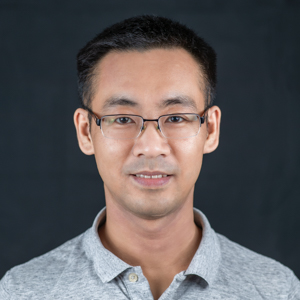
\includegraphics{zhang.jpg}}
\caption{Portrait of Kelei Zhang}
\label{fig}
\end{figure}

Question from Jordan: When I first read this, I missed the bit about you being a photographer. I was confused because it seemed like grad school was a hobby from 2012! :) What is the coolest picture you have taken?
Hi Jordan, thanks for asking the question. I think one of the coolest pictures I had taken was the Big Boy Steam Train. 2019 was the 150th anniversary of Big Boy on the railway. and it was snowing on the day I took the picture. With the team engine and the snowy day, it was quite a beautiful and unforgettable scene. 

Question for Zhang from James Peng: Hi, Zhang, that's awesome to obtain an ability of photography. I'd like to know how you guys capture or design the "composition" of certain moment? For example, in like 3 seconds, you need to decide what moment and how much and what things should be in your frame. This is amazing. How do you guys improve your decision making on the matter? 
Hi James, this is a very good question. I think the most important thing to take a good picture is to learn your camera and master the basic operation. Photography is split into different fields: portraiture, landscape, event, studio, action, etc. I think your question is more about event and action/sports photography where the person has to capture the subject very quickly and also compose perfectly. Well, that almost never happens. For these situations, either the photographer take a series of pictures to capture then select the best one, or they pre compose and wait for the moment. Sometimes, they sit still hours after hours, just like snipers. When they have a clear image, they usually crop to make a better composition. 
